%% LaTeX Beamer presentation template (requires beamer package)
%% see http://bitbucket.org/rivanvx/beamer/wiki/Home
%% idea contributed by H. Turgut Uyar
%% template based on a template by Till Tantau
%% this template is still evolving - it might differ in future releases!

\documentclass{beamer}

\mode<presentation>
{
\usetheme{Darmstadt}

\setbeamercovered{transparent}
} 

\usepackage[english]{babel}
\usepackage[latin1]{inputenc}

% font definitions, try \usepackage{ae} instead of the following
% three lines if you don't like this look
\usepackage{mathptmx}
\usepackage[scaled=.80]{helvet}
\usepackage{courier}
\usepackage{graphicx}
\usepackage{subfigure}
\DeclareGraphicsExtensions{.pdf,.png,.jpg}


\usepackage[T1]{fontenc}


\title{Taking Multi-Object Tracking to the Next Level: People, Unknown Objects, and Carried Items}

%\subtitle{}

% - Use the \inst{?} command only if the authors have different
%   affiliation.
%\author{F.~Author\inst{1} \and S.~Another\inst{2}}
\author{Review by Igor Bogoslavskyi}

% - Use the \inst command only if there are several affiliations.
% - Keep it simple, no one is interested in your street address.
\institute[Universities of]
{
Department Of Computer Science\\
Albert Ludwigs University Freiburg\\
e-mail: bogoslai@informatik.uni-freiburg.de}

\date{2.02.2013}

\begin{document}

\begin{frame}
\titlepage
\end{frame}

\section{Motivation}
%slide 1
\begin{frame}
\frametitle{Motivation} 
\begin{itemize}
  \item Tracking objects in the moving scene is an important task in mobile robotics
\end{itemize}

\begin{center}
  \includegraphics[width=8cm]{image-intro.jpg}
\end{center}

\end{frame}

% slide 2
\begin{frame}
\frametitle{} 
\begin{itemize}
  \item Previously only \emph{tracking-by-detection} approaches. These need pre-trained detector models.
  \item It is important to recognize and track other objects in peoples' surroundings.
  \item Methods that can detect and track also novel object types and learn models for them on-line are needed.
\end{itemize}
\begin{center}
  \includegraphics[width=7.5cm]{motivation_items.jpg}
\end{center}
\end{frame}

\section{Problem Description}
%slide 3
\begin{frame}
\frametitle{Problem Description} 
\begin{itemize}
  \item The problem of detecting novel objects is not trivial.
  \item To do that one has to answer an even harder question - \emph{what is an object}.
  \item This itself involves segmenting object from the video stream input.
\end{itemize}
\end{frame}



%slide 8
\subsection{3D Model}
\begin{frame}
\frametitle{3D Model Representation (Generalized Christmas Tree)} 

\begin{center}
  \includegraphics[width=10cm]{3D_model.pdf}
\end{center}
\begin{itemize}
  \item The model is composed of a vertical axis and several layers of equally spaced horizontal rays.
  \item  Along each ray, 3D points are stored in distance histogram.
\end{itemize}
\end{frame}

\section{Tracking-Before-Detection}
\subsection{Overview}
%slide 4
\begin{frame}
\frametitle{Tracking-Before-Detection Approach} 
\begin{center}
  	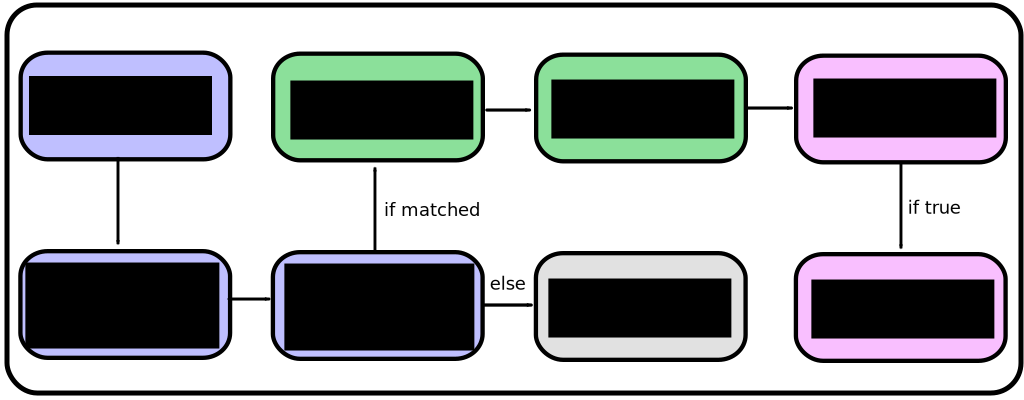
\includegraphics[width=10cm]{overview.pdf}
	\end{center}
\end{frame}


\subsection{Tracking Before Detection Approach}
\begin{frame}
\frametitle{Extracting Regions of Interest (ROIs)} 


  \begin{itemize}
  	\item Project the 3D points within 2m height corridor onto the ground plane.
  	\item Take 2D histogram of these points.
  	\item Remove regions that continuously extend beyond height of 2m to exclude walls and other elevated objects. 
  	\item Threshold the histograms and group to connected components via 8-neighborhood.
  \end{itemize}
\begin{center}
  \includegraphics[width=6cm]{histogram.pdf}
  \end{center}
\end{frame}


%slide 5
\subsection{Tracking Before Detection Approach}
\begin{frame}
\frametitle{Segmentation Into Individual Objects} 


  \begin{itemize}
  	\item Problem: people walking close to each other are still connected in the ground projection.
  	\item Smooth and segment the original histogram via Quick Shift algorithm.
  	\item The result is a segmentation of the ROIs into individual objects.
  \end{itemize}
\begin{center}
  \includegraphics[width=5cm]{histogram.jpg}
  \includegraphics[width=5cm]{image-045.jpg}
  \end{center}
\end{frame}

%slide 7
\begin{frame}
\frametitle{Data Association With Tracked Objects} 

Associating ROIs with existing tracks.
\begin{itemize}
  \item Match newly segmented ROIs to each track's ROI from previous frame.
  \item Match is successful if the over-union of the ROIs' ground projection footprints is over 50\%.
  \item Start a new track for all ROIs that cannot be associated.
\end{itemize}
\end{frame}


%slide 9
\begin{frame}
\frametitle{Match and Update the Model} 

\begin{itemize}
  \item Once the ROI is matched to previous frames, we want to match and update the model.
  \item Match the GCT from current frame to GCT from previous frames via ICP.
  \item After the model were matched we want to update current model to store as much as possible information about the tracked object.
\end{itemize}
\begin{center}
  \includegraphics[width=4cm]{registration.jpg}
\end{center}
\end{frame}

%slide 10
\begin{frame}
\frametitle{Object Classification and Tracking} 

\begin{itemize}
  \item Pass the newly generated track to person/non-person detector. 
  \item Evaluate the detector only for a small region around the back-projected segmented 3D points.
  \item No further classification needed for current object.
\end{itemize}
\end{frame}

%slide 11
\begin{frame}
\frametitle{Pedestrian Model} 
\begin{columns}[T]
    \begin{column}{.7\textwidth}
		\begin{center}
		 	\begin{itemize}
			  \item The 3D model is constantly refined to provide as much detail as possible.
			  \item Compare the on-line model to a learned statistical shape of pedestrians (right image)
			  \item Detect deviations, that cannot be explained by variation in GCT model.
			\end{itemize}
		\end{center}
    \end{column}
    \begin{column}{.3\textwidth}
    	\includegraphics[width=2.5cm]{pedestian_model.jpg}
    \end{column}
\end{columns}
\end{frame}


%slide 12
\begin{frame}
\frametitle{Carried Item Segmentation} 
Carried item segmentation is based on Conditional Random Fields.
	\begin {itemize}
		\item Unary potentials are based on the Bhattacharyya distance between the distance histograms of the on-line tracked and learned model rays.
		\item A weighting function in a direction orthogonal to the ground plane was added to unary potential as a prior that carried items are usually not in the leg area.
		\item Pairwise potentials - contrast-sensitive Potts model based on image colors was used.
	\end{itemize}
\end{frame}

%slide 13
\section{Results}
\subsection{Datasets}
\begin{frame}
\frametitle{Datasets}
\begin{center}
  	\includegraphics[width=6.5cm]{shopping_example.jpg}
\end{center}
\begin{itemize}
	\item Three different datasets captured from a stereo camera setup
 were used:
	\begin{itemize}
		\item BAHNHOF: 999 frames with 5193 pedestrian annotations.
		\item SUNNY DAY: 354 frames with 1867 pedestrian annotations.
		\item SHOPPING: over 540 frames with 3398 pedestrians annotations.
\end{itemize}
\end{itemize}
\end{frame}

%slide 14
\subsection{Pedestrian Tracking Performance}
\begin{frame}
\frametitle{Pedestrian Tracking Performance} 
\begin{center}
  	\includegraphics[width=8.5cm]{dataset_graphs.pdf} \newline
  	\includegraphics[width=4.25cm]{dataset_graphs_small.pdf}
\end{center}
\end{frame}

%slide 15
\subsection{Object Tracking Performance}
\begin{frame}
\frametitle{Object Tracking Performance} 
\begin{center}
	\includegraphics[width=7cm]{table.pdf}
\end{center}
\begin{itemize}
	\item Tracking the unknown objects listed in Tab. 8
	\item 6060 frames of video material. 
\end{itemize}
\end{frame}

%slide 16
\begin{frame}
\frametitle{Pedestrian/Object Tracking Examples} 
\begin{center}
  	\includegraphics[width=4cm]{objects1.jpg} \hspace{0.5cm}
  	\includegraphics[width=4cm]{objects2.jpg}
\end{center}
\begin{center}
  	\includegraphics[width=4cm]{objects3.jpg} \hspace{0.5cm}
  	\includegraphics[width=4cm]{objects4.jpg}
\end{center}

\end{frame} 

%slide 17
\subsection{Carried Item Detection Performance}
\begin{frame}
\frametitle{Carried Item Detection Performance} 
Comparison of segmentation results with the labeled data.
\begin{center}
  	\includegraphics[width=8cm]{carried.pdf}
\end{center}

\end{frame}

%slide 18
\begin{frame}
\frametitle{Carried Item Detection Examples} 
\begin{center}
  	\includegraphics[width=4cm]{items1.jpg} \hspace{0.5cm}
  	\includegraphics[width=4cm]{items2.jpg}
\end{center}
\begin{center}
  	\includegraphics[width=4cm]{items3.jpg} \hspace{0.5cm}
  	\includegraphics[width=4cm]{items4.jpg}
\end{center}

\end{frame}

%slide 19
\section{Conclusion}
\begin{frame}
\frametitle{Conclusion} 
\begin{itemize}
	\item The approach is based on \emph{tracking-before-detection} paradigm as opposed to older \emph{detection-before-tracking} one.
	\item This leads to the possibility to detect and track unknown objects.
	\item The presented 3D model allows not only achieving state-of-the-art tracking performance but also analyzing the shape of tracked person in more detail to detect carried items while running the system on-line.
\end{itemize}
\end{frame}

%slide 20
\begin{frame}
\frametitle{Questions?} 
\begin{center}
  	\includegraphics[width=7cm]{questions.jpg}
\end{center}
\end{frame}



\end{document}
